\section{Methodology}

\begin{figure}[tb]
    \begin{minipage}{0.48\textwidth}
      \centering
      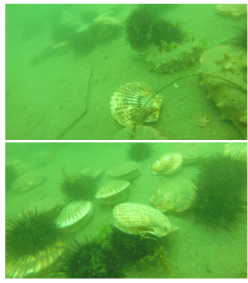
\includegraphics[width=.7\linewidth]{figures/pre-processing.png}
      \caption{Input underwater Image}
      \label{Fig:PreProcessing}
    \end{minipage}\hfill
    \begin{minipage}{0.48\textwidth}
      \centering
      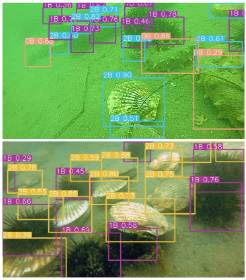
\includegraphics[width=.7\linewidth]{figures/post-processing.png}
      \caption{Enhanced Image with recognized objects}
      \label{Fig:PostProcessing}
    \end{minipage}
\end{figure}

\subsection{Data Collection}

In this project publicly available underwater image datasets will be used,
such as the Underwater Object Detection Dataset (UODD) 
\parencite{jiangUnderwaterSpeciesDetection2021}
\footnote{UODD dataset is available at
\url{https://github.com/LehiChiang/Underwater-object-detection-dataset}}.
These datasets contain a diverse range of underwater scenes, including various
flora, fauna, and man-made objects, providing a comprehensive basis for testing
and comparison, along with annotations labeled in MS COCO format.

Given the inherent challenges of underwater imaging,
such as varying light conditions and turbidity, images will undergo
pre-processing to enhance quality and consistency.
Techniques like color correction, contrast adjustment,
and noise reduction will be applied to mitigate environmental effects on
image quality, like shown in \parencite{tengUnderwaterTargetRecognition2020}
and \parencite{pengUshapeTransformerUnderwater2023}.

\subsection{Model Selection and Development}

\begin{APAitemize}
    \item \textbf{CNNs}: Initial experiments will focus on conventional
     CNN architectures, which have proven effective in basic underwater object
     detection tasks.
     These models will serve as a benchmark for comparing more advanced
     architectures. % Add citations

    \item \textbf{Residual Networks (ResNets)}: Given their ability to train
     deeper networks by mitigating the vanishing gradient problem,
     ResNets will be explored for their potential to improve recognition
     accuracy in complex underwater scenes. % Add citations

     \item \textbf{Transformers}: The study will also incorporate Transformer
     models, which utilize self-attention mechanisms, to examine their
     effectiveness in capturing the spatial relationships of objects in
     underwater images. % Add citations
\end{APAitemize}

\subsection{Implementation}

The project will employ Python as the primary programming language,
leveraging its extensive ecosystem and the ease of finding pre-implemented
models along with Jupyter notebook to help the visualization of data.
For model implementation and training, I will utilize deep learning
libraries such as TensorFlow and PyTorch.
Experiments will be conducted on a laptop equipped with an Nvidia GPU
to facilitate efficient model training and evaluation.

\subsection{Evaluation Criteria}

The evaluation of the various models will use common indicators like accuracy,
precision, recall and F1 score along with the confusion matrix
to determine the effectiveness of each model in correctly identifying and
classifying underwater objects.

\begin{figure}[ht]
    \begin{tabular}{l|l|c|c|c}
        \multicolumn{2}{c}{}&\multicolumn{2}{c}{Prediction outcome}&\\
        \cline{3-4}
        \multicolumn{2}{c|}{}&Positive&Negative&\multicolumn{1}{c}{Total}\\
        \cline{2-4}
        \multirow{2}{*}{Actual values}& Positive & $TP$ & $FN$ & $P'$\\
        \cline{2-4}
        & Negative & $FN$ & $TN$ & $N'$\\
        \cline{2-4}
        \multicolumn{1}{c}{} & \multicolumn{1}{c}{Total} & \multicolumn{1}{c}{$P$} & \multicolumn{    1}{c}{$N$} & \multicolumn{1}{c}{}\\
    \end{tabular}
    \caption{Confusion Matrix used for model evaluation}
    \label{Tab:confMatrix}
\end{figure}

\begin{equation}
    F1 = \frac{2*Precision*Recall}{Precision+Recall} = \frac{2*TP}{2*TP+FP+FN}
\end{equation}

Additionally, computational efficiency, measured in terms of training time
and inference speed, will be considered to assess the practicality
of deploying these models in real-world applications.

The performance of each architecture will be compared to establish
their relative strengths and weaknesses in underwater object recognition.
This analysis will also explore the impact of varying dataset complexities
and environmental conditions on model performance.

\FloatBarrier